
\section*{Code implementation }
The code has been written in Python , while back in 2016 the researcher 
decided to write the code for training the Net in LUA .
So first of all we understand the code written in LUA by the authors and 
after we decide to translate it in Python . 
The main reason why we do it is that the code was deprecated after about 10 years (
especially the library ) and for us was not possible to try to train the Net 
ourself . 
Talking about the Datasets they were also not reacheable because the hyperlink redirect 
to a website not existing anymore .
So we try to develop a solution in which we train the Net with the same concept described 
before but using different Datasets .  
Also the trained weights cannot be adapted to the new solution that we develop ,
so we decide so re-train the Network from zero for about 200 epochs .
After the 200 epochs we decide to stop the training because it was taking too long .
\\
The code in subdivided in different part and diffent .ipynb file .
The first one is "1) dataset usage.ipynb" in which is possible the are two example 
on how to load Bird and Flowers Dataset using the module "gan\_t2i" and store it in HDF5 format 
other than using a Dataloader on this datasets .
The second file is "2) CLIP - Fine Tuning.ipynb" in which is shown how to load the CLIP model 
(ViT-B/32) and to train it (we use an already trained CLIP network to extract text features )
The Third file is "3.2) COLAB GAN example.ipynb" . In this file we combine all the 
module that we develop until now . 
First of all we decide which network we would like to train between : "Vanilla\ GAN", "GAN\_INIT\_CLS" 
and "WGAN" . 
After this part we download the weights related to the CLIP Network used to extract 
the text features and also the model itself .
What about the Dataset initially it is stored in HDF5 format but this time is also 
transformed and normalized other than tokenized .
After this section we create the training, validation and test dataloaders and check the 
outcome size of the CLIP model feature related to text and images .
And then depending on the Newtwork that we would like to train 
we define it and define the embedding projection dimension that in our case is 128 .
Finally after this long pre-processing and initilization part we can decide if start to train
the Net using the correspondent Algoritm from zero or from a specific checkpoint ( which corrispond
to the weights ) loading it in the Model . 
The result on the GAN model after 186 epochs of training from scratch are not enough to prodoce a result 
which correspond to the description given by the text , that's due to the fact that the Net is too complex 
and in fact to achieve a satisfactory result, at least 600 epochs are necessary, 
as the original paper also specifies.
Besides the visualization factor it's possible to observe that the loss related to the Discrimination and 
Generator part tend to move in the right direction , in fact the Generator loss especially in the WGAN model
tend do descrease (minimize) and the Discriminator loss it's maximizing it's values as well as described 
in the Min-Max optimization formula .
\\
\section*{WGAN on FASHION-MNIST Dataset}
We try also to conduce some experiments on training the Net addressing the problem to other Datasets 
such as Fashion MNIST dataset ( keras.datasets.fashion\_mnist ) .
\\
So in general the WGAN employs the Wasserstein distance 
to define a value function with properties theoretically superior  
compared to the one introduced in the original GAN paper .
As seen before to verify that the Discriminator (critic) respects the 
1-Lipschitz requirement, the authors implemented weight clipping. 
However, this technique might lead to problems like as low convergence 
in deep critics and other unwanted phenomena.
WGAN-GP substitutes weight clipping with a "gradient penalty." 
This variant includes a loss term to keep the L2 norm of the discriminator 
gradients around a set value, allowing for smoother training . But it's based 
on the Algoritm \ref{alg:WGAN} flow-chart described in the section related to the 
Architectures.
\\
\subsection*{Data Preparation}
The dataset used is the FASHION-MNIST dataset , in which each 
sample is a 28x28 grayscale pixel image with values 
normalized in the range [-1,1] . 
The label related to the image will not be used in this case 
to train the WGAN .
\\
\subsection*{Discriminator Net}
In this case the Discriminator use a Zero Padding layer to transform 
the input image (28,28,1) into a shape of (32,32,1) and other
4 Convolutional Block to transform it in (16,16,64) $\rightarrow$  ( 8, 8, 128)
$\rightarrow$ (4, 4, 256) $\rightarrow$ (2, 2, 512)
Leaky Relu is used as activation function .
\\
The Convolutional Block is composed of 2D Convolutional Kernel 
and depending on the parameters a Normalization and dropout layer .
The output shape of the discriminator is one value that rappresent 
the "real" or "fake" classification of the input image, 
indicating whether the image is from the real dataset or 
generated by the Generator.
\subsection*{Generator Net} 
The Genetor Net use the upsample\_block(..) function 
to handle the upsampling process by increasing the spatial 
dimensions of the input with UpSampling2D, followed by a Conv2D layer .
Depending on the parameter it may also include BatchNormalization 
and a specific activation function (like LeakyReLU or Tanh) 
to introduce non-linearity and improve training stability other
than a Dropout layer to prevent overfitting.
The Generator starts by taking a noise vector as input, 
transforming it through a Dense layer into a tensor of shape 
(4, 4, 256). 
The data is then passed through three Upsampling blocks .
In the same way in the second block, the shape changes from (8, 8, 128) 
to (16, 16, 64), again using UpSampling2D and Conv2D, 
with BatchNormalization and LeakyReLU applied.
The third one  increases the shape from (16, 16, 64) 
to (32, 32, 1) by applying UpSampling2D and Conv2D 
to reduce the channels to 1, followed by a Tanh activation 
to ensure the output is in the correct range.
Lastly , a Cropping2D layer is applied to reduce the spatial 
dimensions from (32, 32) to (28, 28) to generate the image .
\subsection*{WGAN-GP MODEL}
The model overrides the \texttt{keras.Model} module and overrides the 
\texttt{train\_step} function derived from the model. 
The model consists of a discriminator and a generator. 
The discriminator processes real and fake images, 
while the generator creates fake images from random noise.
The model is initialized with specific hyperparameters like 
\texttt{latent\_dim} (dimension of the random input to the generator),
\texttt{discriminator\_extra\_steps} (extra steps to train the 
discriminator), and 
\texttt{gp\_weight} (weight for the gradient penalty).

\subsection*{Gradient Penalty Function}
The model uses a custom gradient penalty function, 
which helps to enforce the Lipschitz constraint by calculating the norm of the gradient of the discriminator's output with respect to interpolated images. This is added to the discriminator's loss.

\subsection*{Training Step}
During training, we work using batches of 512. 
The discriminator is updated multiple times per generator 
step (3 extra steps are typically used). 
For each discriminator step, fake images are generated 
based on the noise vector. The discriminator is used 
two times on the fake and real images, and the discriminator's 
loss is computed based on the function passed (we will define it after), 
obtaining \texttt{d\_cost}. 
Based on the real and fake images, we compute the gradient penalty. 
Finally, the total discriminator loss (\texttt{d\_loss}) 
is computed as : 
\\
\texttt{d\_loss = d\_cost + gp * self.gp\_weight}.
\\
The generator is trained after the discriminator. 
The generator's loss is computed based on the discriminator's output, 
and it depends on the generated images coming from the Generator 
Network. The generator loss function will be defined after.
Each model (discriminator and generator) is updated using their 
respective optimizers. The training process alternates between 
updating the discriminator and the generator, with 
the gradient penalty ensuring stability.
The optimizers used for this task are the same and correspond to 
Adam with a learning rate of 0.0002.
\\
\subsection*{Discriminator Loss}
The discriminator loss is simple and computes the mean of the 
batch values obtained on real and fake images, as well 
as the difference between them.
\subsection*{Generator Loss}
The generator loss is straightforward because it is 
the negative mean of the logits (unnormalized output values 
produced by the model) for fake images, 
pushing the generator to produce images that the discriminator 
classifies as real. A positive score suggests 
the image is real, and a negative score suggests it is fake. 
By minimizing this negative loss, the generator is maximizing 
the discriminator’s score for the generated images, 
effectively making the fake images more "realistic" in the 
eyes of the discriminator.
\subsection*{Training time}
The network is trained for around 30 epochs, with a noise dimension 
of 128. After each epoch, a callback generates and saves a number of 
images based on the latent noise vector as PNG files. 
The values from the generator are in the range of [-1, 1] due 
to the \texttt{Tanh} activation function, so these values 
are rescaled to the range [0, 255] to be saved correctly. 
We perform the inverse process to normalize the pixels in 
the range [-1, 1] when preparing each sample of the dataset.
\\
\begin{figure}[h!]
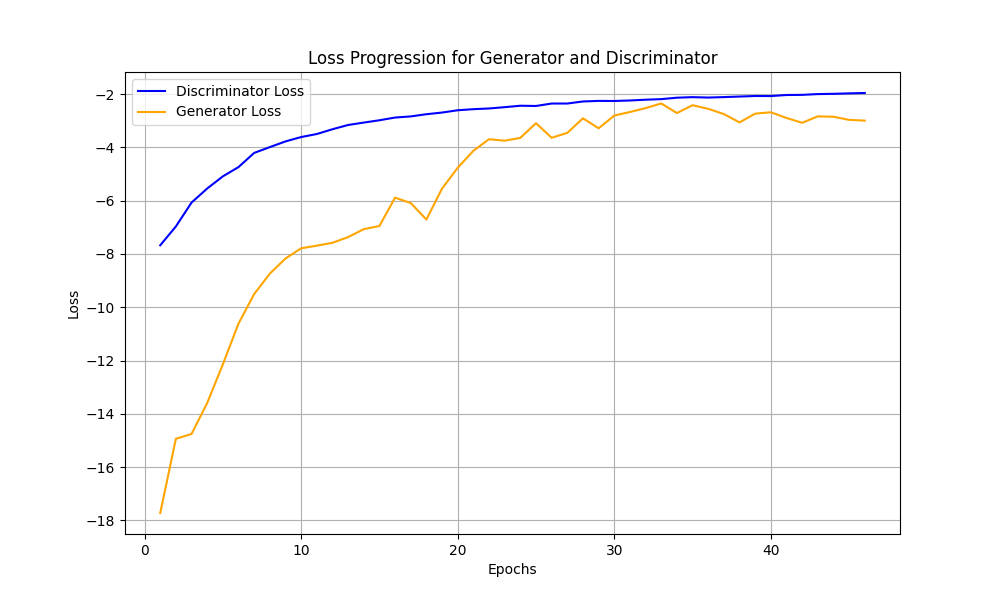
\includegraphics[width=80mm]{loss_D_G.png}
\caption{Discriminator Loss during Training (WGAN)}
\end{figure}
\\
In general , especially because the problem has been simplified with respect 
to the previous one , after only 50 epochs we can appreciate good result in term of 
reconstruction of image related to the MNIST datasets .
And thanks to the gradient penalty term we can generalize the enough to obtain 
a good reconstruction also on "zero-shot" data coming from the same dataset . 
\\
The visual results of the model's performance after various epochs are shown below. 
As it is possible to observe, the reconstructions generated by the "Generator" become 
increasingly coherent with the noise given as input as the epochs increase.

\begin{figure}[h!]
    \centering
    \caption{Grid of generated images at different epochs}
    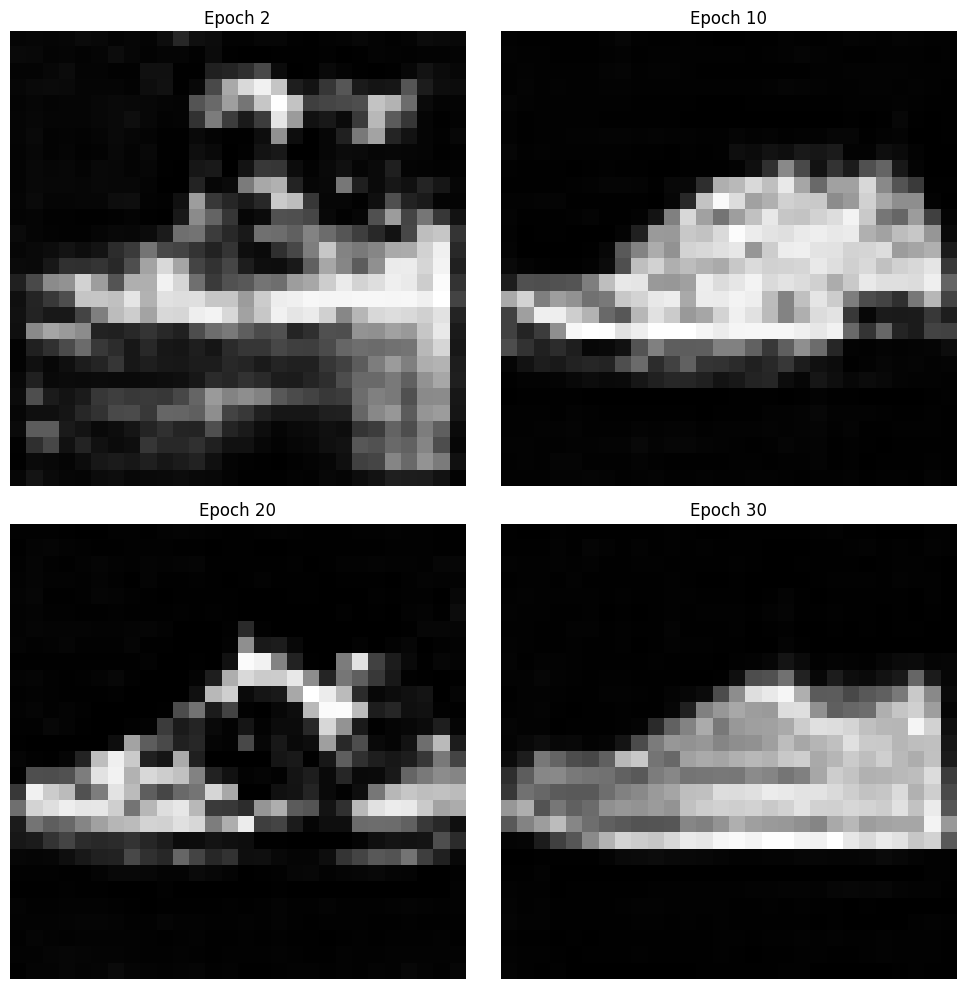
\includegraphics[width=0.4\textwidth]{images/Epochs.png}
    \label{fig:grid_plot}
\end{figure}